
  
\documentclass[letterpaper, 12pt]{article}

\usepackage{natbib}
\usepackage{hyperref}
\usepackage{graphicx}
\usepackage{amsmath}
\usepackage[dvipsnames]{xcolor}
\usepackage[format=plain,justification=RaggedRight, labelfont=bf]{caption}
\usepackage[style=plain,floatrowsep=qquad]{floatrow}
\usepackage{sectsty}
\usepackage[compact]{titlesec}
\usepackage{aas_macros}
\usepackage{amsmath}
\usepackage[charter]{mathdesign}
\usepackage[margin=1in]{geometry}
\usepackage{fancyhdr}
\usepackage{float}
\usepackage{wrapfig}

\pagestyle{plain}
%\pagestyle{fancy}
%\fancyhf{}
\rhead{Corey Brummel-Smith}
\lhead{Enriching the Universe with Metals from the First Stars}

\hypersetup{pdfpagemode={UseOutlines},
  bookmarksopen,
  colorlinks,
  linkcolor={Black},
  citecolor={Black},
  urlcolor={RoyalBlue}}

\bibliographystyle{apj}

\newcommand*{\eg}{{e.\,g.,}\xspace}
\newcommand*{\ie}{{i.\,e.,}\xspace}

\newcommand{\todo}[1]{{\color{red} TODO: #1}}

%%%%%%%%%%%%%%%%%%%%%%%%%%%%%%%%%%%%%%%%%%%%%%%%%%%%%%%%%%%%%%%%%%%%%%%%%%%%%%%%

% Alter some LaTeX defaults for better treatment of figures:
% See p.105 of "TeX Unbound" for suggested values.
% See pp. 199-200 of Lamport's "LaTeX" book for details.
% General parameters, for ALL pages:
%\renewcommand{\topfraction}{0.9}    % max fraction of floats at top
%\renewcommand{\bottomfraction}{0.8} % max fraction of floats at bottom
%
% Parameters for TEXT pages (not float pages):
\setcounter{topnumber}{2}
\setcounter{bottomnumber}{2}
\setcounter{totalnumber}{2}             % 2 may work better
\setcounter{dbltopnumber}{2}            % for 2-column pages
%\renewcommand{\dbltopfraction}{0.9} % fit big float above 2-col. text
%\renewcommand{\textfraction}{0.07}  % allow minimal text w. figs
%
% Parameters for FLOAT pages (not text pages):
%\renewcommand{\floatpagefraction}{0.7}  % require fuller float pages
%
% N.B.: floatpagefraction MUST be less than topfraction !!
%\renewcommand{\dblfloatpagefraction}{0.7} % require fuller float pages

% 12pt section/subsection headers
\allsectionsfont{\fontsize{12}{15}\selectfont}

\begin{document}
%%%%%%%%%%%%%%%%%%%%%%%%%%%%%%%%%%%%%%%%%%%%%%%%%%%%%%%%%%%%%%%%%%%%%%%%%%%%%%%%%%%%%%%%
% BEGIN Personal Statement
%%%%%%%%%%%%%%%%%%%%%%%%%%%%%%%%%%%%%%%%%%%%%%%%%%%%%%%%%%%%%%%%%%%%%%%%%%%%%%%%%%%%%%%%

\thispagestyle{fancyplain}
\rhead{Corey Brummel-Smith}
\lhead{Personal Statement}

As I studied physics throughout undergrad I became possessed with a curiosity to understand the nature of the universe on astronomical scales. Through studying physics and computer science, I became increasingly interested in computational physics simulations, and their power to investigate the complex, non-linear, problems in modern astrophysics such as star formation and the evolution of the universe as a whole. This set me on a path to pursue my goal of obtaining a Ph.D. in physics, and take the necessary steps to become a professor and conduct research at a university.

My drive to learn about numerical simulations led me to my first research position with Dr. David Collins at Florida State University (FSU), where I was introduced to Enzo: An Adaptive Mesh Refinement Code for Astrophysics. Using Enzo simulations, I investigated the magnetic field structure in turbulent molecular clouds to explain how magnetic fields can modulate and suppress star formation. Another key component of this research was studying how magnetic field structure affects the polarization of foreground dust emission, which is important for understanding the polarization of the cosmic microwave background and the cosmology of our universe \citep{Clark2015}. This research helped me develop the technical skills necessary to succeed as a researcher and computational physicist. For this research, the Center for Undergraduate Research and Academic Engagement at FSU awarded me with a grant and invited me to present my work at the President’s Showcase of Undergraduate Research Excellence. This allowed me to hone my ability to speak about physics and astronomy with a non-technical audience; a skill which will benefit me in the future as I strive toward my goal of becoming a professor and science communicator.

At the end of my undergraduate career, I searched for graduate schools that would allow me to dive deeper into my quest to become a computational astrophysicist. This led me to work with Dr. John Wise in the Computational Cosmology Group at the Center for Relativistic Astrophysics at Georgia Tech. My research with John began by investigating what appeared to be a triggered star formation event in one of his previous Enzo simulations. I discovered a couple of major problems in the simulations. To fix the bugs, I needed to learn about the inner workings of Enzo in much greater detail. Over the last two years, I have learned an incredible amount about the Enzo code; from the details of interpolation and flux correction, to how to choose optimal parameters for certain simulations. Knowledge of these details is important, not only to fix problems as they arise but also to know how to design new simulations, such as the ones in this proposal. I have attended two Enzo developer workshops where I have contributed to the codebase, reviewed new code modifications, and helped teach new users how to use and edit the code. I am now a contributing author on the most recent Enzo publication, which documents recent changes to the code \citep{ENZO2019_JOSS}.

In December of 2018, I applied to the Kavli Summer Program in Astrophysics (KSPA), hosted at the Center for Computational Astrophysics (CCA). I was selected to attend this summer school along with 16 other distinguished graduate students from all around the world. With my mentors, Daisuke Nagai, Yuan Li, and Irina Zhuravleva, we worked on a project where I created and analyzed mock x-ray images of simulated galaxy clusters. By comparing mock observations of simulated clusters, and real observations of existing ones, we were able to test the effectiveness of our observational techniques in understanding feedback physics from active galactic nuclei (AGN). This unique project helped bridge a gap between simulations and observations. Most importantly, this work has led to an ongoing collaboration, and we have now extended this project far beyond the scope of what we were able to achieve at the KSPA.
In the following year, because of my work at the KSPA, one of Daisuke’s collaborators, requested my help in preparing a White Paper for The Decadal Survey on Astronomy and Astrophysics. I created mock x-ray images of AGN feedback in a simulated galaxy cluster using different telescope instrument models. With these images, we demonstrated how a next-generation telescope with an effective area larger than the Chandra observatory, would allow us to probe the physics of AGN feedback on smaller scales than ever before. Specifically, we showed we would be able to resolve shock waves and other perturbations that would otherwise be hidden in Chandra images with a realistic exposure time \citep{WP_Ruszkowski2019}. 

In the winter of 2018, I traveled to the Kavli Institute for the Physics and Mathematics of the Universe in Tokyo Japan to attend the conference "Stellar Archeology as a Time Machine for the first stars." There I presented my research on metal-transport from a supernova into a nearby molecular cloud found in one of Dr. Wise's simulations of the formation of the first stars. This research is what sparked my idea to study triggered star formation in a systematic and controlled way. Not only was this a great opportunity to share my research with others, but it also allowed me to meet many experts in the field of stellar archeology and the first stars and continue to develop a professional network. At the conference, I learned a lot of valuable information about the state of the field that has helped guide the development of my research plan for this proposal.

All Ph.D. students enrolled in the School of Physics at Georgia Tech are required to be a teaching assistant (TA) for the undergraduate physics courses in their first year. For many, this is a tedious distraction from coursework and research, but for me, this was an eye-opening and fun endeavor. I taught recitation sections where students would solve context-rich physics problems in small groups. My job was to help students when they had trouble and did not understand concepts taught in their lectures. I did this by asking thought-provoking questions to help guide them without giving away answers. I never knew how much I would enjoy teaching and sparking the students' interest in physics. There is something about spreading the knowledge that I love with others that brings me joy and satisfaction. This is one of the primary reasons why I want to become a physics or astronomy professor in the future.

These experiences have strengthened my drive to become a professor and continue researching unsolved problems in astronomy, such as, what were the properties of the first stars and galaxies, and how can we learn about them today? Through graduate schooling and research experience, I’ve developed the professional and technical skills necessary to succeed as a computational physicist and achieve these goals.

\noindent{\textbf{Graduate study timeline:} \\
I began my graduate studies in Fall 2017. As is the norm for most physics grad students on the Ph.D. track at Georgia Tech, I took the core physics courses in my first year. In Spring 2018, I joined Dr. Wise's Computational Cosmology group and also received my M.S. in physics from Georgia Tech. In the next two years, I continued research with Dr. Wise while taking one to two astrophysics courses per semester. I will select a Ph.D. committee and give my thesis proposal at the end of my third year (Summer 2020). Upon passing the thesis proposal exam, I will be admitted as a Ph.D. candidate. I will then continue research until I complete my dissertation. On average, students in the School of Physics take approximately six years to complete their Ph.D. Using this as an estimate, I expect to graduate in Spring 2023.}

\pagebreak

%%%%%%%%%%%%%%%%%%%%%%%%%%%%%%%%%%%%%%%%%%%%%%%%%%%%%%%%%%%%%%%%%%%%%%%%%%%%%%%%%%%%%%%%
% END Personal Statement
%%%%%%%%%%%%%%%%%%%%%%%%%%%%%%%%%%%%%%%%%%%%%%%%%%%%%%%%%%%%%%%%%%%%%%%%%%%%%%%%%%%%%%%%

%%%%%%%%%%%%%%%%%%%%%%%%%%%%%%%%%%%%%%%%%%%%%%%%%%%%%%%%%%%%%%%%%%%%%%%%%%%%%%%%%%%%%%%%
% BEGIN Science/Technical/Management Section
%%%%%%%%%%%%%%%%%%%%%%%%%%%%%%%%%%%%%%%%%%%%%%%%%%%%%%%%%%%%%%%%%%%%%%%%%%%%%%%%%%%%%%%%
%\setcounter{page}{1}
\thispagestyle{fancyplain}
\rhead{Corey Brummel-Smith}
\lhead{Science/Technical/Management Section}

\section{Introduction}

The elements that comprise everything we see around us, in fact, nearly everything from the second row of the periodic table down, did not exist before the formation of the first stars. Understanding the first stars is not just important for understanding our cosmic origins; they are crucial in understanding the formation of galaxies throughout cosmic time, and the evolution of the early universe as a whole. The difficulty is when we look toward the edge of the observable universe, all these first stars are too faint, and closer to home, they are already dead. Thus, studying them observationally is not currently possible. These, so-called, Population III (Pop III) stars are generally thought to be much more massive than regular stars, on the order of 100 $M_{\odot}$, with some possibly as large as 1000 $M_{\odot}$. The only connection we have to them are the clues they have imprinted on the second generation of stars, by enriching them with their metals. When Pop III stars explode, they enrich the environment with metals formed in their cores and their supernovae, whose remnants can later collapse to form new, metal-poor (Pop II) stars \citep{Chiaki2019}. Pop II stars have more typical masses, living longer lives and may still exist today in places like the galactic halo and ultra-faint dwarf galaxies (UFDGs) \citep{Kirby2008}. One of the goals of stellar archeology is to infer the properties of the first stars by observing the distribution and metallicities of their long-lived descendants. However, since individual Pop II stars may be enriched by multiple Pop III progenitors, it is often impossible to infer the precise masses and metallicities of the first stars. We will address this problem with two separate types of numerical simulations. Each type of simulation will provide a unique connection between Pop III and Pop II stars. In the first project, we will investigate whether supernova induced star formation can produce second-generation, metal-poor stars enriched by a single progenitor. In the second project, we will track metals from multiple Pop III stars in cosmological simulations, and determine exactly how many Pop III stars enrich the second-generation stars. \textbf{Ultimately, this work will provide a deeper understanding of the transition away from a metal-free universe, and allow us to constrain the masses, metallicities, and distribution of the first stars.}

\subsection*{Carbon Enhanced Metal-Poor Stars}

In some cases, the metallicity of the second stars could be set entirely by the yields of the Pop III stars. The stellar life-cycle produces more metals with each successive generation, and thus, today, we see stars with a metal abundance orders of magnitude larger than that of the stars in the early universe. Since the overall metal abundance of the universe continually grows over time, metallicity is related to stellar age, making metal-poor stars the fossils of the early universe, and within their chemical composition, they hold the secrets of the first stars. Carbon-enhanced metal-poor (CEMP) stars are of particular interest because of their iron deficiency, showing they exist early before Type-Ia supernovae provide the bulk of the iron content in galaxies. These stars are divided into three groups based on their iron and carbon abundances. Group II and III stars have lower metallicity than Group I and are comprised of CEMP-no stars, which are CEMP stars with no overabundance of s-process elements \citep{Maeder2015}. CEMP-no stars are of particular interest to us because a detailed analysis of their chemical composition strongly supports the hypothesis that these stars formed out of pregalactic clouds enriched by the first-generation stars \citep{Yoon2016}. However, the details of their formation and their connection to the first stars is not fully understood. \cite{Yoon2016} also point out that more than one class of progenitors for Group II and Group III stars exist, and yet-to-be suggested sites of star formation and metal enrichment may account for the contrasts between Group II and III. \textbf{In our first project, we will investigate a new formation channel, fueled by triggered star formation, that could help explain the origins and differences between Group II and Group III CEMP-no stars. In project 2, we will investigate whether these differences arise from the number of Pop III progenitors.}

% \begin{wrapfigure}{L}{\textwidth}
%   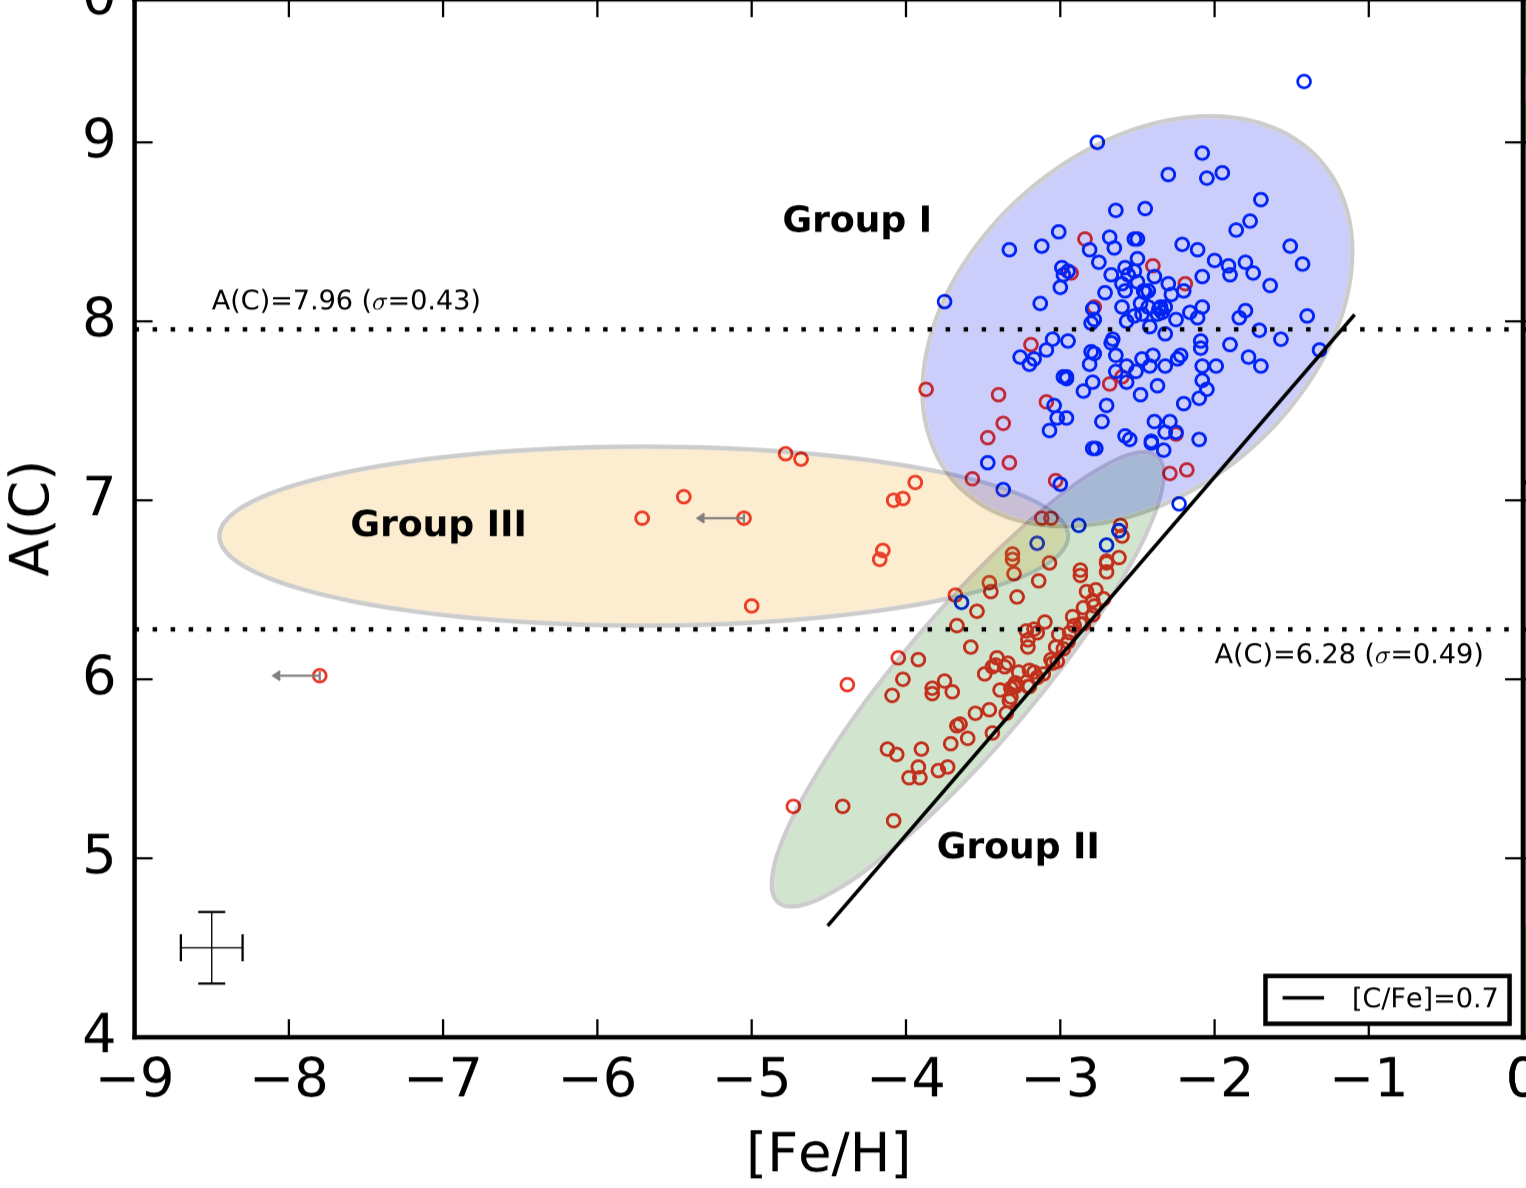
\includegraphics[width=0.55\textwidth]{figures/cemp_groups}
%   \caption{CEMP star groups}
%   \label{fig:cemp_groups}    
% \end{wrapfigure}

\section{Proposed Work}
The overall goal of our two projects will be to use numerical simulations to track metals from the supernova remnants of individual Pop III stars, all the way to their final resting place in the stellar nurseries of the second-generation stars. Our proposed work will provide a quantitative connection between the first stars and their metal-poor descendants, which will allow us to constrain the properties of actual Pop III stars, from observations of CEMP stars and the metal-poor galaxies in which they live. Each project investigates different spatial and temporal scales. In project 1, we focus on a particular star formation mechanism involving a single Pop III star in its local parsec-scale environment. In project 2, we study how metals from many Pop III stars are transported throughout the universe on cosmological scales. 

\subsection*{Project 1: Supernova Induced Formation of the Second Stars}
\label{sec:tsf}

\textbf{Motivation:} Simulations indicate that the typical formation channel for the second-generation stars is the internal enrichment (IE) scenario \citep{Chiaki2019}. IE occurs when a Pop III star explodes, enriching its host dark matter halo with metals for the first time, and the supernova remnant collapses to form new stars in tens of Myrs, which is much longer than the lives of massive Pop III stars. For reference, a 40 $M_\odot$ Pop III star has a main sequence lifetime of 3.86 Myr \citep{Schaerer2002}. This means it is possible and -- maybe even likely -- that Pop II stars will be seeded by multiple Pop III progenitors, making it difficult to infer the metal yields and masses of the individual Pop III stars. However, if all the metals in a cluster of Pop II stars were to come from a single progenitor, one could infer the yields and mass of the progenitor by measuring the metallicity of the cluster. Enrichment by a single progenitor could happen by triggered star formation. If a Pop III star explodes in close proximity to a molecular cloud, it could mechanically crush it into gravitational collapse, or heat the surrounding environment enough for the increased pressure to induce gravitational instability. A diagram of this is shown in Figure \ref{fig:tsf}. After the cloud becomes gravitationally unstable, stars will form in roughly the free-fall time of the cloud. This would typically be on the order of millions of years rather than several tens of millions. Therefore, there would not be enough time for other Pop III stars to contaminate the protostellar cloud.

% \begin{wrapfigure}{R}{0.6\textwidth}
%   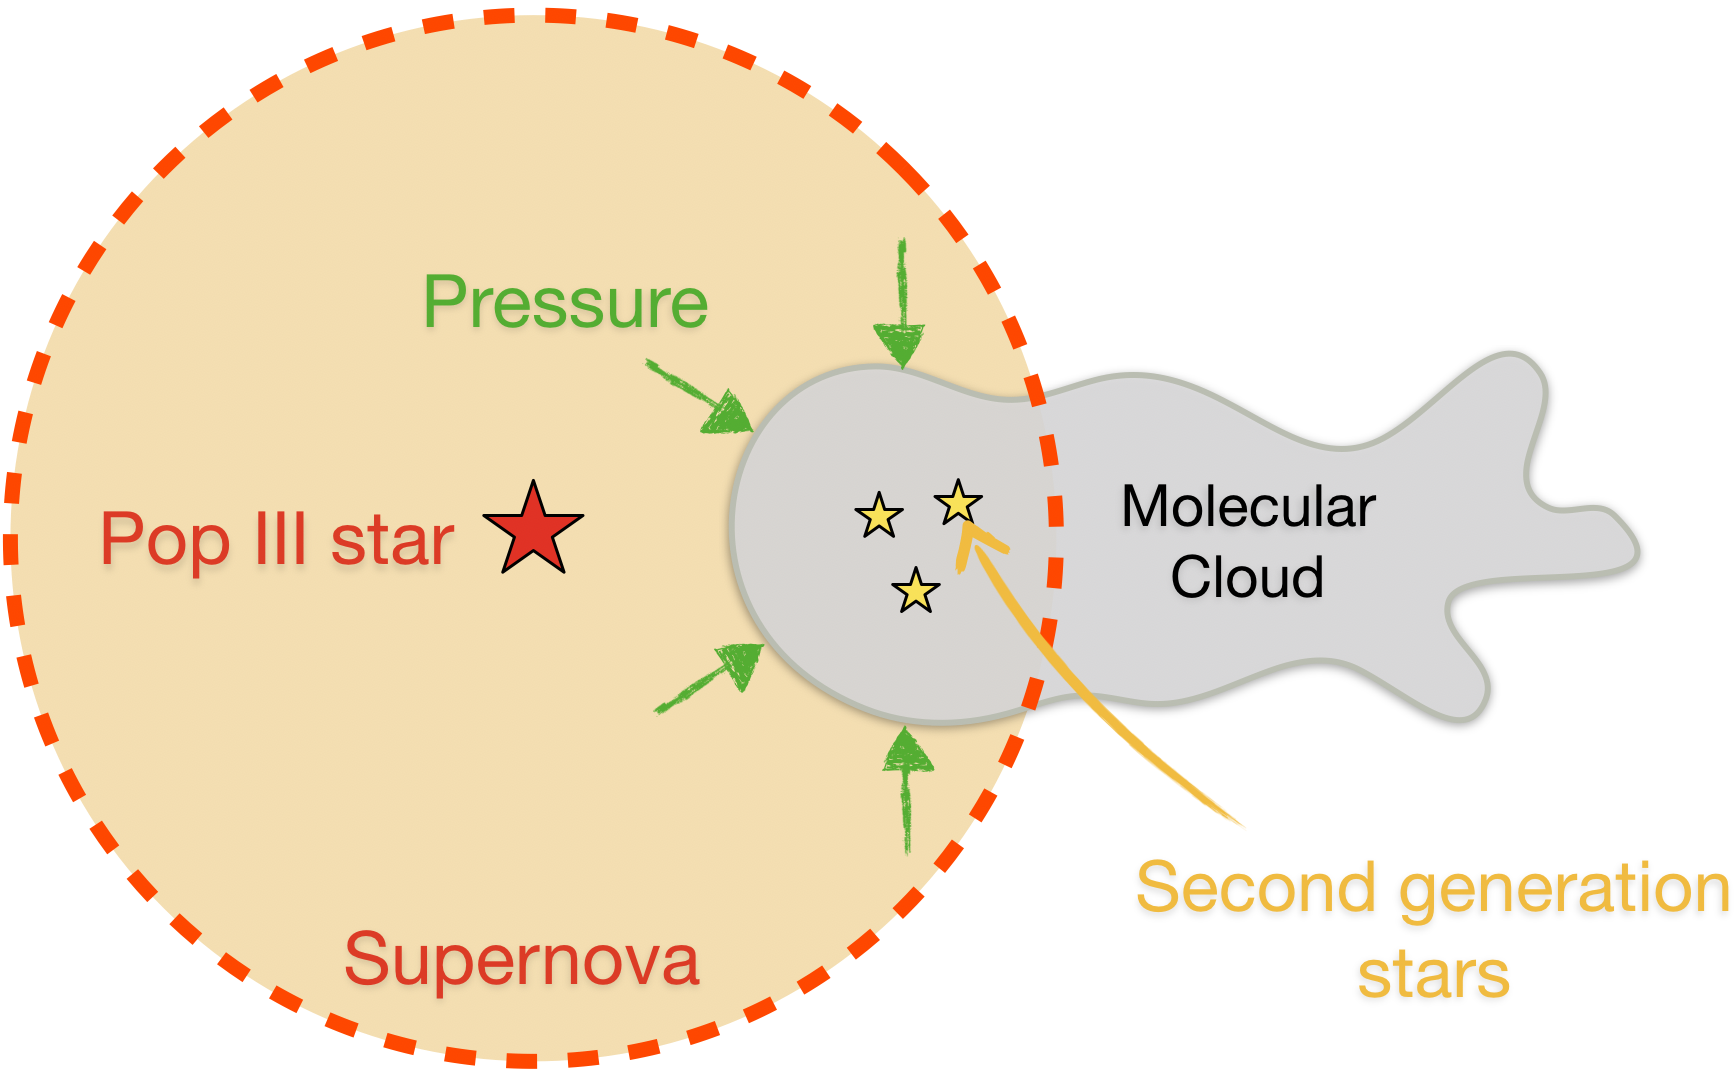
\includegraphics[width=0.6\textwidth]{figures/tsf2}
%   \caption{Diagram of the triggered star formation scenario.}
%   \label{fig:tsf}
% \end{wrapfigure}

\begin{wrapfigure}{R}{0.55\textwidth}
  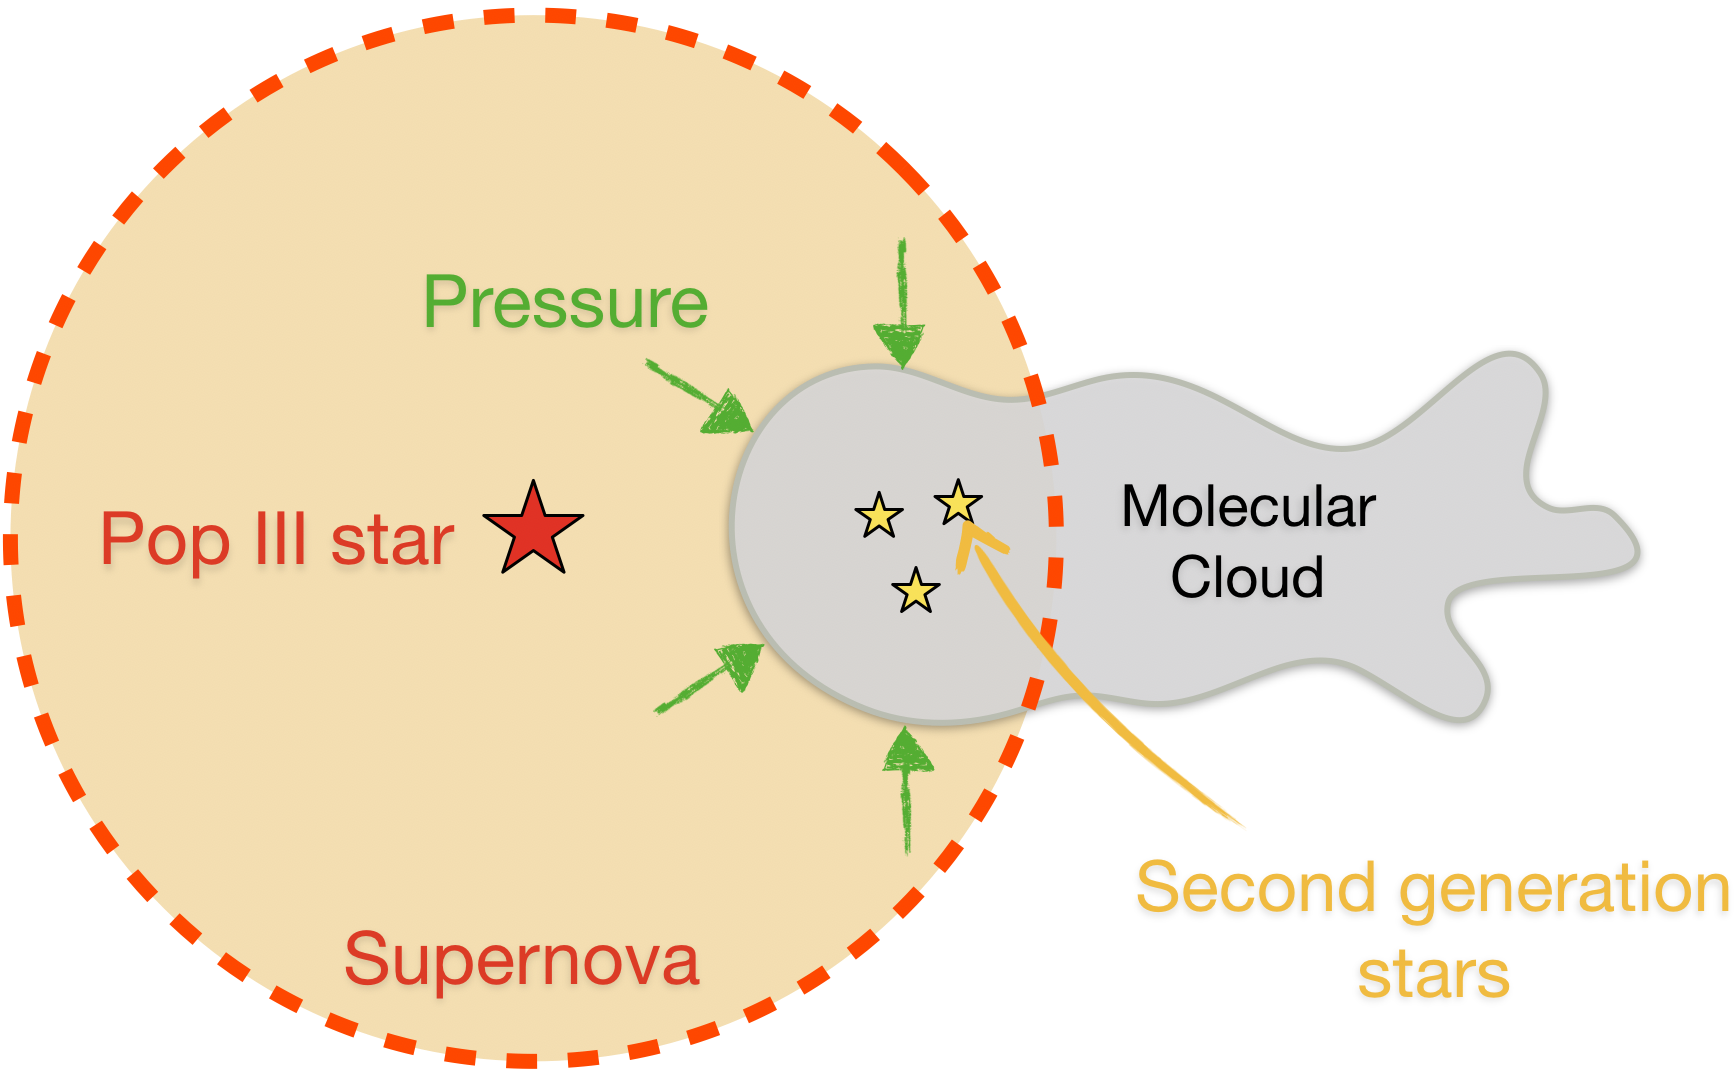
\includegraphics[width=\textwidth]{figures/tsf2}
  \caption{Triggered star formation diagram.}
  \label{fig:tsf}
\end{wrapfigure}

\textbf{Research plan:} We will study triggered star formation and its role in the formation of metal-poor stars using numerical hydrodynamic simulations with radiative and supernova feedback. These simulations will be run with Enzo: an adaptive mesh refinement (AMR) code for astrophysics \citep{Bryan2014}. Enzo is an excellent code to use because it solves the ideal magneto-hydrodynamic equations for the gas density, energy, momentum, and magnetic fields, while also simulating the effects of stellar radiation feedback and radiative cooling. Enzo is also integrated with the Grackle chemistry and cooling library \citep{Smith2017}, which will allow us to model the formation and destruction of $H_2$, as well as many other chemical species that affect the heating and cooling rates of the chemically-enriched gas. All of these processes are important to accurately model star formation in a physically realistic manner. 

By systematically studying triggered star formation, we can determine the conditions necessary for this to occur in the early universe, and most importantly, identify a causal link between the mass and yields of individual progenitor Pop III stars and the observable properties of their metal-poor descendants. We will run at least 36 realizations of these simulations spanning a parameter space consisting of the mass of the progenitor, the mass of the molecular cloud, and the distance between the cloud and progenitor. This will allow us to determine the optimal conditions for triggered star formation. From these results, we can easily verify our claim that this formation channel occurs on a shorter timescale than typical IE. The most important part of this project will involve studying how metals from the supernova remnant mix into the cloud, which will determine the metallicity of the second-generation stars.

\textbf{Feasibility and previous work:} Multiple studies have shown that triggered star formation via cloud crushing is possible under certain conditions \citep{Melioli2006, Leao2009}, though none have specifically investigated the transfer of metals into the star-forming region. We can, however, gain useful insight from these existing simulations. \cite{Melioli2006} analytically determined when triggered star formation can occur in the parameter space of supernova radius and cloud density. They confirmed their results with hydrodynamical simulations. We will use these results as a guide for constructing our parameter space, but also test cases that would, according to their model, not induce star formation. Not only will this test the robustness and reproducibility of their results, but it may also reveal important differences that could arise from different simulation codes, grid resolutions, cooling models, and explosion energies. Another important difference is our prestellar cloud will be initially metal-free, whereas theirs had an abundance of heavy metals.

\textbf{Analysis:} We will track the gravitational collapse -- or lack thereof -- and determine when star formation occurs by performing various analyses in post-processing. The simplest way to approximately determine when the cloud becomes gravitationally unstable is to measure the ratio of the enclosed mass to the Bonnor-Ebert (BE) mass. It is important to use the BE mass, rather than the Jeans mass because the hot supernova remnant will provide external pressure on the cool molecular cloud. This pressure acts to decrease the critical mass necessary for gravitational collapse leading to the formation of stars.

With each of these simulations, we will analyze the metal transport from the supernova remnant into the cloud, to determine the metallicity of the second-generation stars. We will investigate how the distribution of metallicity as a function of density and radius evolves over time. Once the mixing timescale becomes longer than the free-fall time of the cloud, metals will no longer efficiently mix into the core, and thus, this will determine the resultant metallicity of the subsequent stars. 

\textbf{Outcome:} If metals do not efficiently mix into the cloud, this could potentially explain how the lowest metallicity, CEMP-no stars in Group III formed, and allow us to estimate the properties of their progenitors. If metals mix in more efficiently, this could potentially explain the origin of the higher metallicity CEMP-no stars in Group II. Either way, if the conditions for triggered star formation can be achieved in the early universe, \textbf{these simulations will help explain the existence of the CEMP-no stars via a new formation channel.} These simulations will also provide a direct link between the properties of second-generation stars and \textit{individual} Pop III progenitors. If and when we observe metal-poor stars indicative of a single enrichment event, this would suggest that they could be products of triggered star formation. The results of this work will allow us to determine the properties of the stars that created them.

While triggered star formation could produce Pop II stars enriched by a single progenitor, it is certainly not the only formation channel for metal-poor stars in the local universe. To better determine the properties of the first stars, we must also understand the metal enrichment and the formation of second-generation stars enriched by multiple progenitors.

\subsection*{Project 2: Tracking Metals from Pop III Stars in Cosmological Simulations}
\label{subsec:tracer_particles}

\textbf{Goal:} With this project, we will, for the first time, provide a direct connection between multiple progenitors and their metal-poor descendants by tracking the metals that are uniquely tagged from the supernovae of individual population III stars. Not only will this allow us to report \textit{exactly} how many Pop III stars enrich a given Pop II star cluster, but we will also know the relative fractions that come from each progenitor. Since we will be able to tell the exact mass and metal yields of each Pop III star, we will be able to make predictions about the properties of the progenitors of the actual CEMP-no stars observed in the halo of our galaxy and UFDGs. 

\textbf{Research plan:} To model the star formation process in a realistic, self-consistent manner, we will run a suite of cosmological simulations initialized using MUSIC \citep{Hahn2011}, with the most recent cosmological parameters \cite{Planck2018}. MUSIC allows us to easily initialize "zoom-in" simulations that will highly resolve the galaxies in a large cosmological volume. We will use Enzo for the reasons described in Section \ref{sec:tsf}. Another benefit of this code is by using AMR we can focus the bulk of the computational resources on high-density dark matter halos and star-forming clouds.

However, resolving objects the size of individual stars in such a simulation is not computationally tenable. We, therefore, use a sub-grid model for star formation and feedback. Since the turbulent mixing timescale is typically longer than the free-fall timescale in our simulations, all stars in a cluster will have approximately the same metallicity. Since this proposal is primarily focused on metal enrichment, it is not necessary to resolve individual stars. Stars in the simulation are represented as point particles, advected in a Lagrangian manner, in contrast to the advection of the fluid fields which is done on an Eulerian grid. An important feature of these star particles is they inject energy and momentum back into the grid via heat and radiation pressure. The stars also produce ionizing Lyman-Werner radiation capable of dissociating $H_2$ molecules \citep{Safranek-Shrader2012}. The stars will continue their feedback until they have exhausted their time on the main sequence, at which point they produce a supernova. Unlike previous simulations of Pop III stars \citep[e.g.][]{Smith2015, Chiaki2019}, we will vary the explosion energy depending on the mass of the progenitor. This allows us to simulate different types of explosions from faint supernovae to hypernovae, which produce different metal yields. The lifetimes of the Pop III stars will be determined from \cite{Schaerer2002} and the supernova metal yields will be taken from \cite{Nomoto2006} and \cite{Heger2010}.

When Pop III stars form, their mass will be randomly sampled from an initial mass function (IMF). Since the IMF of the first stars is unknown, we will run four simulations with different IMFs. The functional form will be a power-law with a slope of -1.3 and an exponential cutoff below a characteristic mass \citep{Wise2012}. Our fiducial model will use a characteristic mass of 40 $M_{\odot}$ and only allow core-collapse supernovae. Each additional simulation will have a different characteristic mass and include other types of supernovae (faint, jet, and pair-instability). \textbf{This will allow us to put better constraints on the true IMF.}
 
% \begin{figure}
%   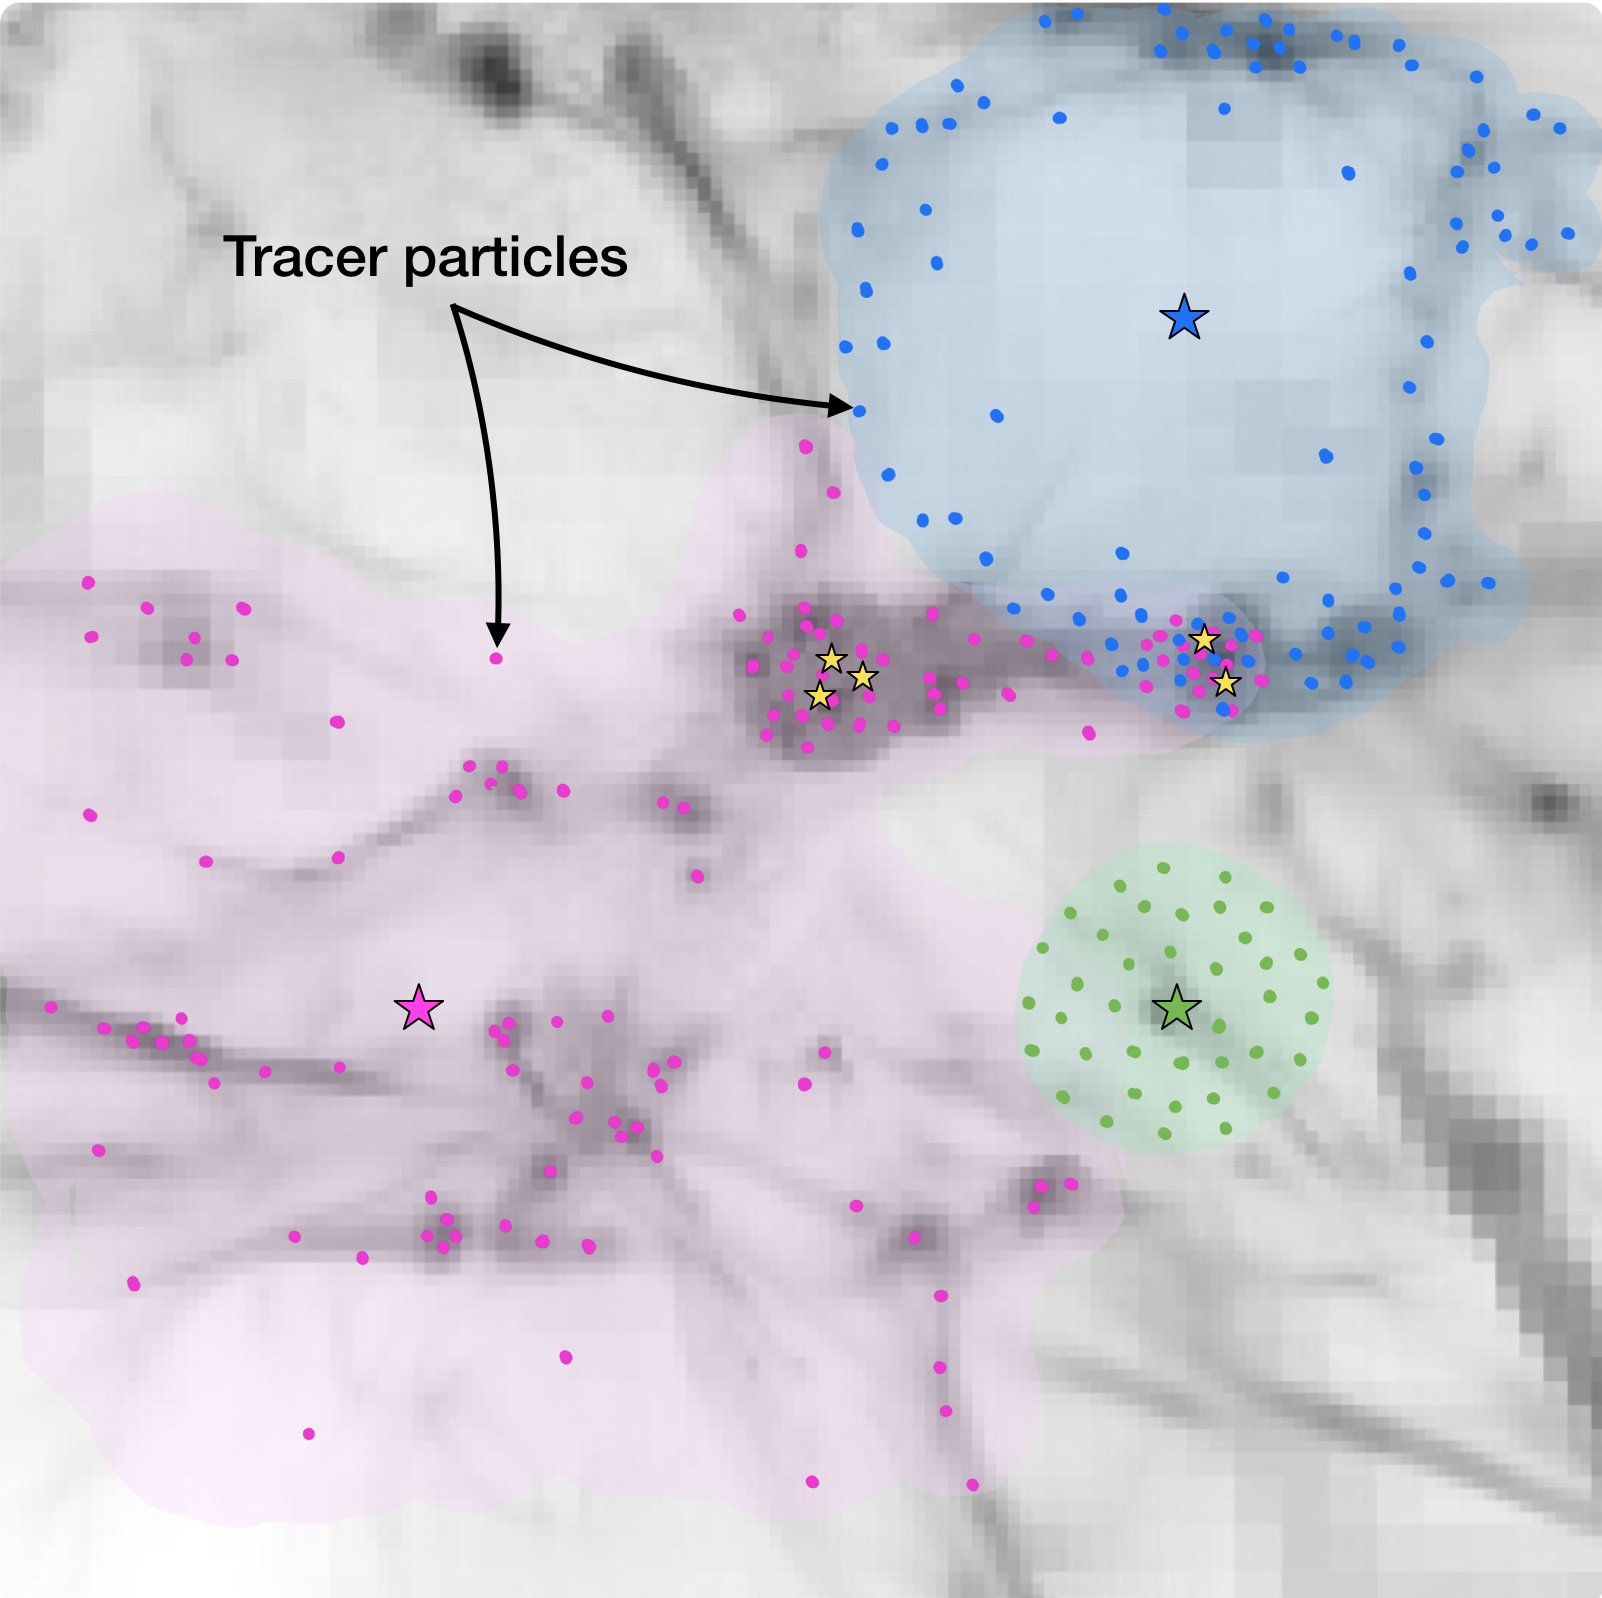
\includegraphics[width=0.58\textwidth]{figures/tracer_final}
%   \caption{Qualitative illustration of metal tracer particles (colored points). Black and white colors represent gas density in an example cosmological simulation. Blue, pink, and green highlighted regions represent metal enrichment from the supernova remnants of Pop III stars (blue, pink and green stars). Gold stars represent potential sites of second-generation star formation. No stars are actually present in the example simulation.}
%   \label{fig:tracer}    
% \end{figure}

\begin{wrapfigure}{R}{0.54\textwidth}
  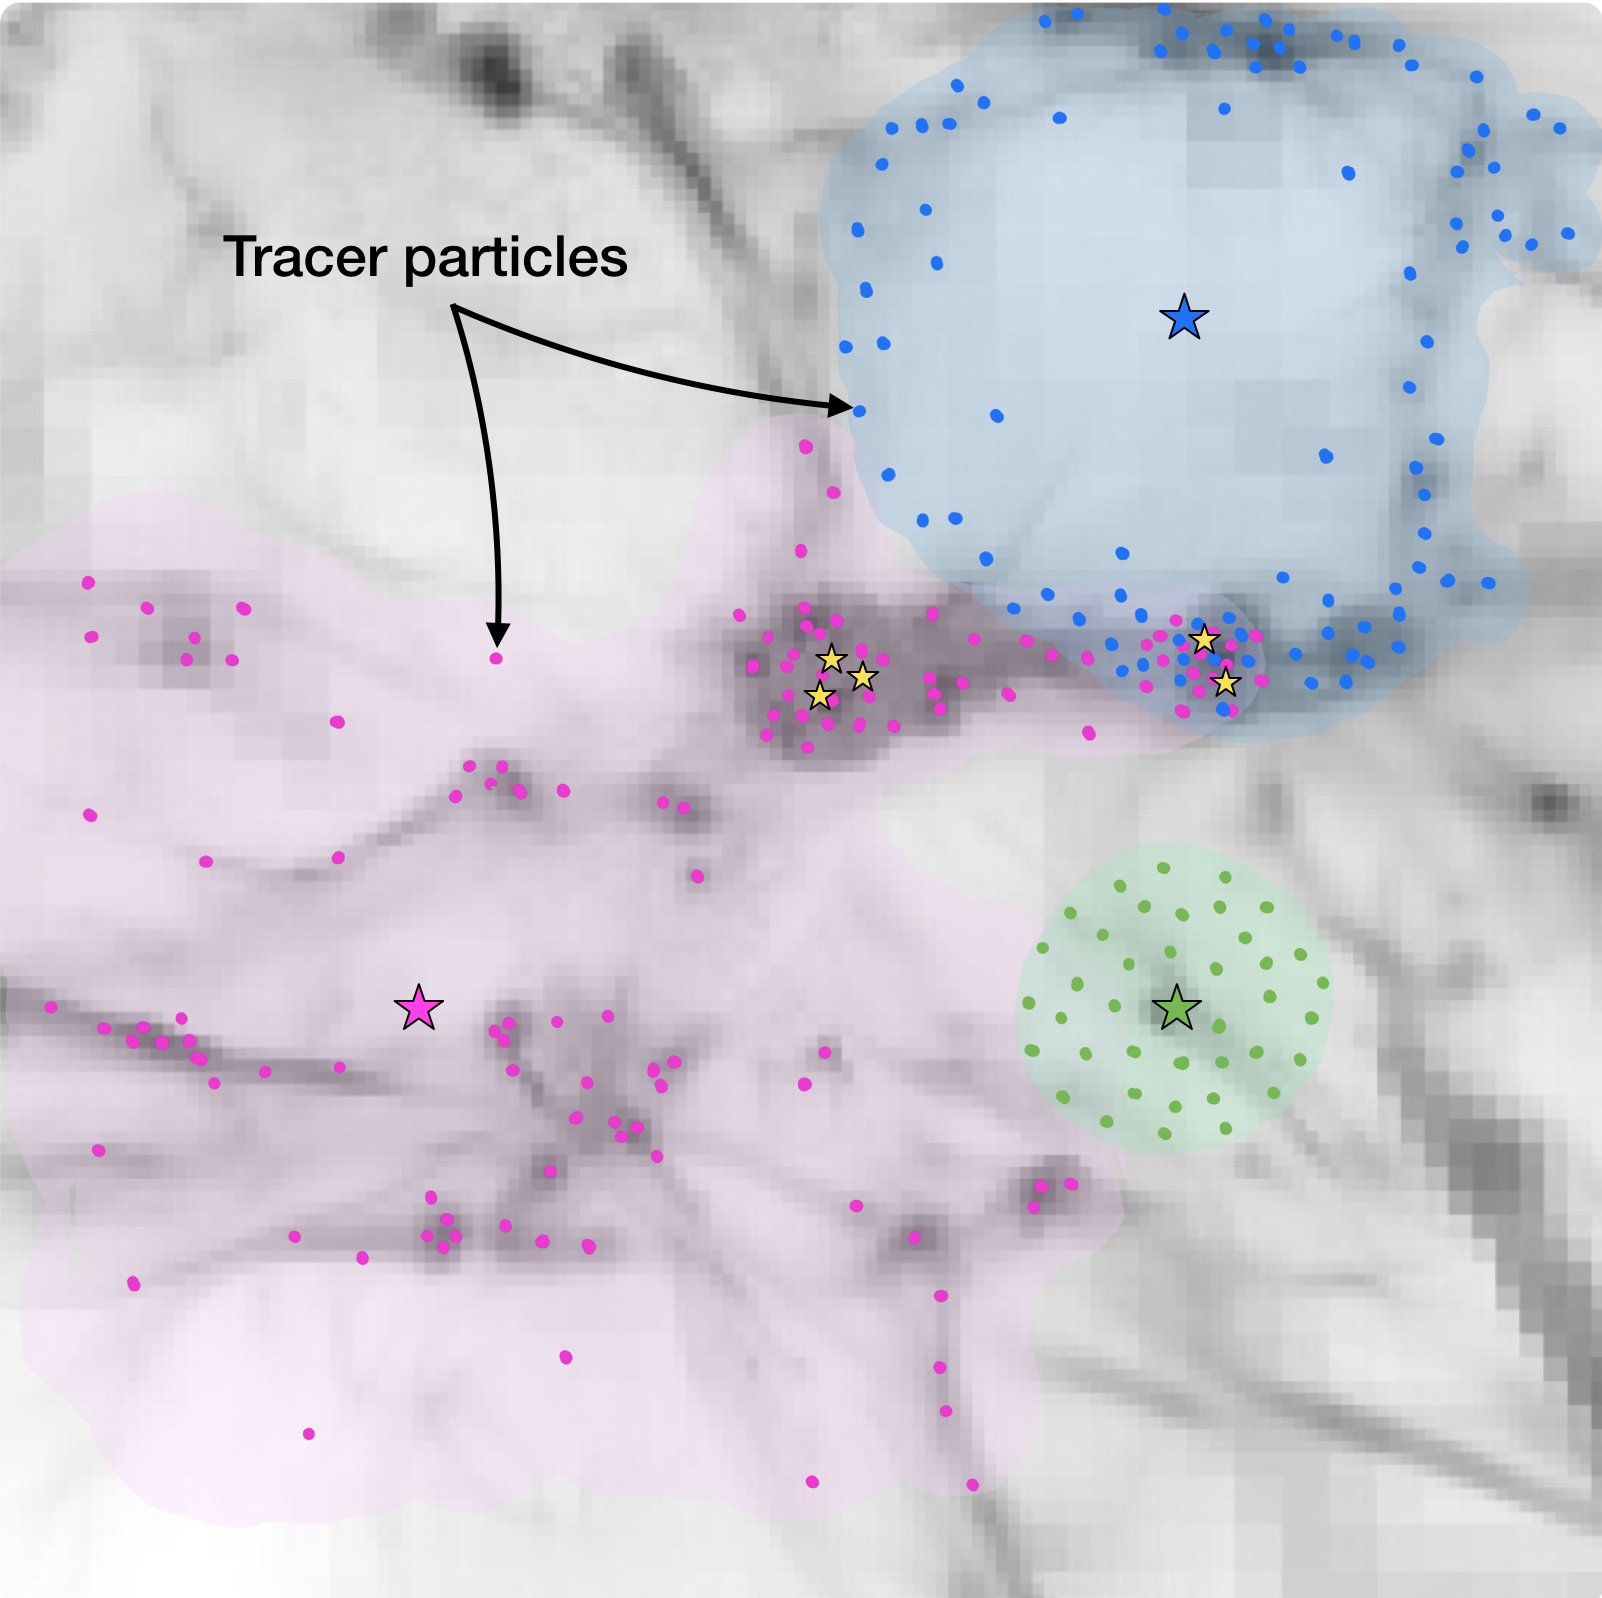
\includegraphics[width=\textwidth]{figures/tracer_final}
  \caption{Qualitative illustration of metal tracer particles (colored points). Black and white colors represent gas density in an example cosmological simulation. Blue, pink, and green highlighted regions represent metal enrichment from the supernova remnants of Pop III stars (blue, pink and green stars). Gold stars represent potential sites of second-generation star formation. No stars are actually present in the example simulation.}
  \label{fig:tracer}    
\end{wrapfigure}

When the Pop III stars explode, energy, momentum, and metals are deposited onto the grid in a spherical region around the star. However, unlike any previous cosmology simulation involving the chemical connection between Pop III stars and UFDG progenitors, we will inject tracer particles into the supernovae. These massless tracer particles will have identifiers unique to the Pop III star that produced them. They will be advected with the gas flow from the supernovae, and thus, will track the proliferation of the metals from their source. Over time, these particles will collapse with the metals into high-density regions where the second-generation stars will form. Due to the unique identifiers of the tracer particles, \textbf{we will be able to tell exactly which Pop III stars produce the metals that enrich the second-generation stars, and how many progenitors they have.} A qualitative illustration of this is shown in figure \ref{fig:tracer}. This is of great importance because it will provide a direct connection between the first and second stars. With a large enough sample of Pop III stars in the simulation, we will be able to make statistically significant conclusions about how often metal-poor stars are enriched by one or more progenitors and the fraction of metals coming from each. To ensure we have a sufficient number of dark matter halos and Pop III stars, we will choose a box size of 1 co-moving Mpc, a root grid resolution of $256^3$, with a maximum of 12 levels of refinement. This gives a minimum cell size of 0.1 proper pc. Given this simulation domain, we would expect on the order of 500 Pop III stars to form. For the sake of argument, if one assumes a second-generation star-forming region has, at most, 5 distinct progenitors, this leaves a minimum of 100 individual sites to investigate the formation of metal-poor stars.

\textbf{Outcome:} Not only will these simulations allow us to study the number of progenitors seeding the second stars, but they will also allow us to determine where the progenitors lived. Pop II stars are either enriched internally by progenitors within the same halo or externally by progenitors in a neighboring halo. Our tracer particles will show which of these channels occurs more frequently, and the differences in metal enrichment between the two scenarios. By including multiple types of supernovae with different metal yields, we can determine how Group II and Group III CEMP-no stars are formed, and why there are two distinct groups.

%%% ORIGINAL PLACEMENT TRACER PARTICLES FIGURE %%%%
%\begin{figure}
%  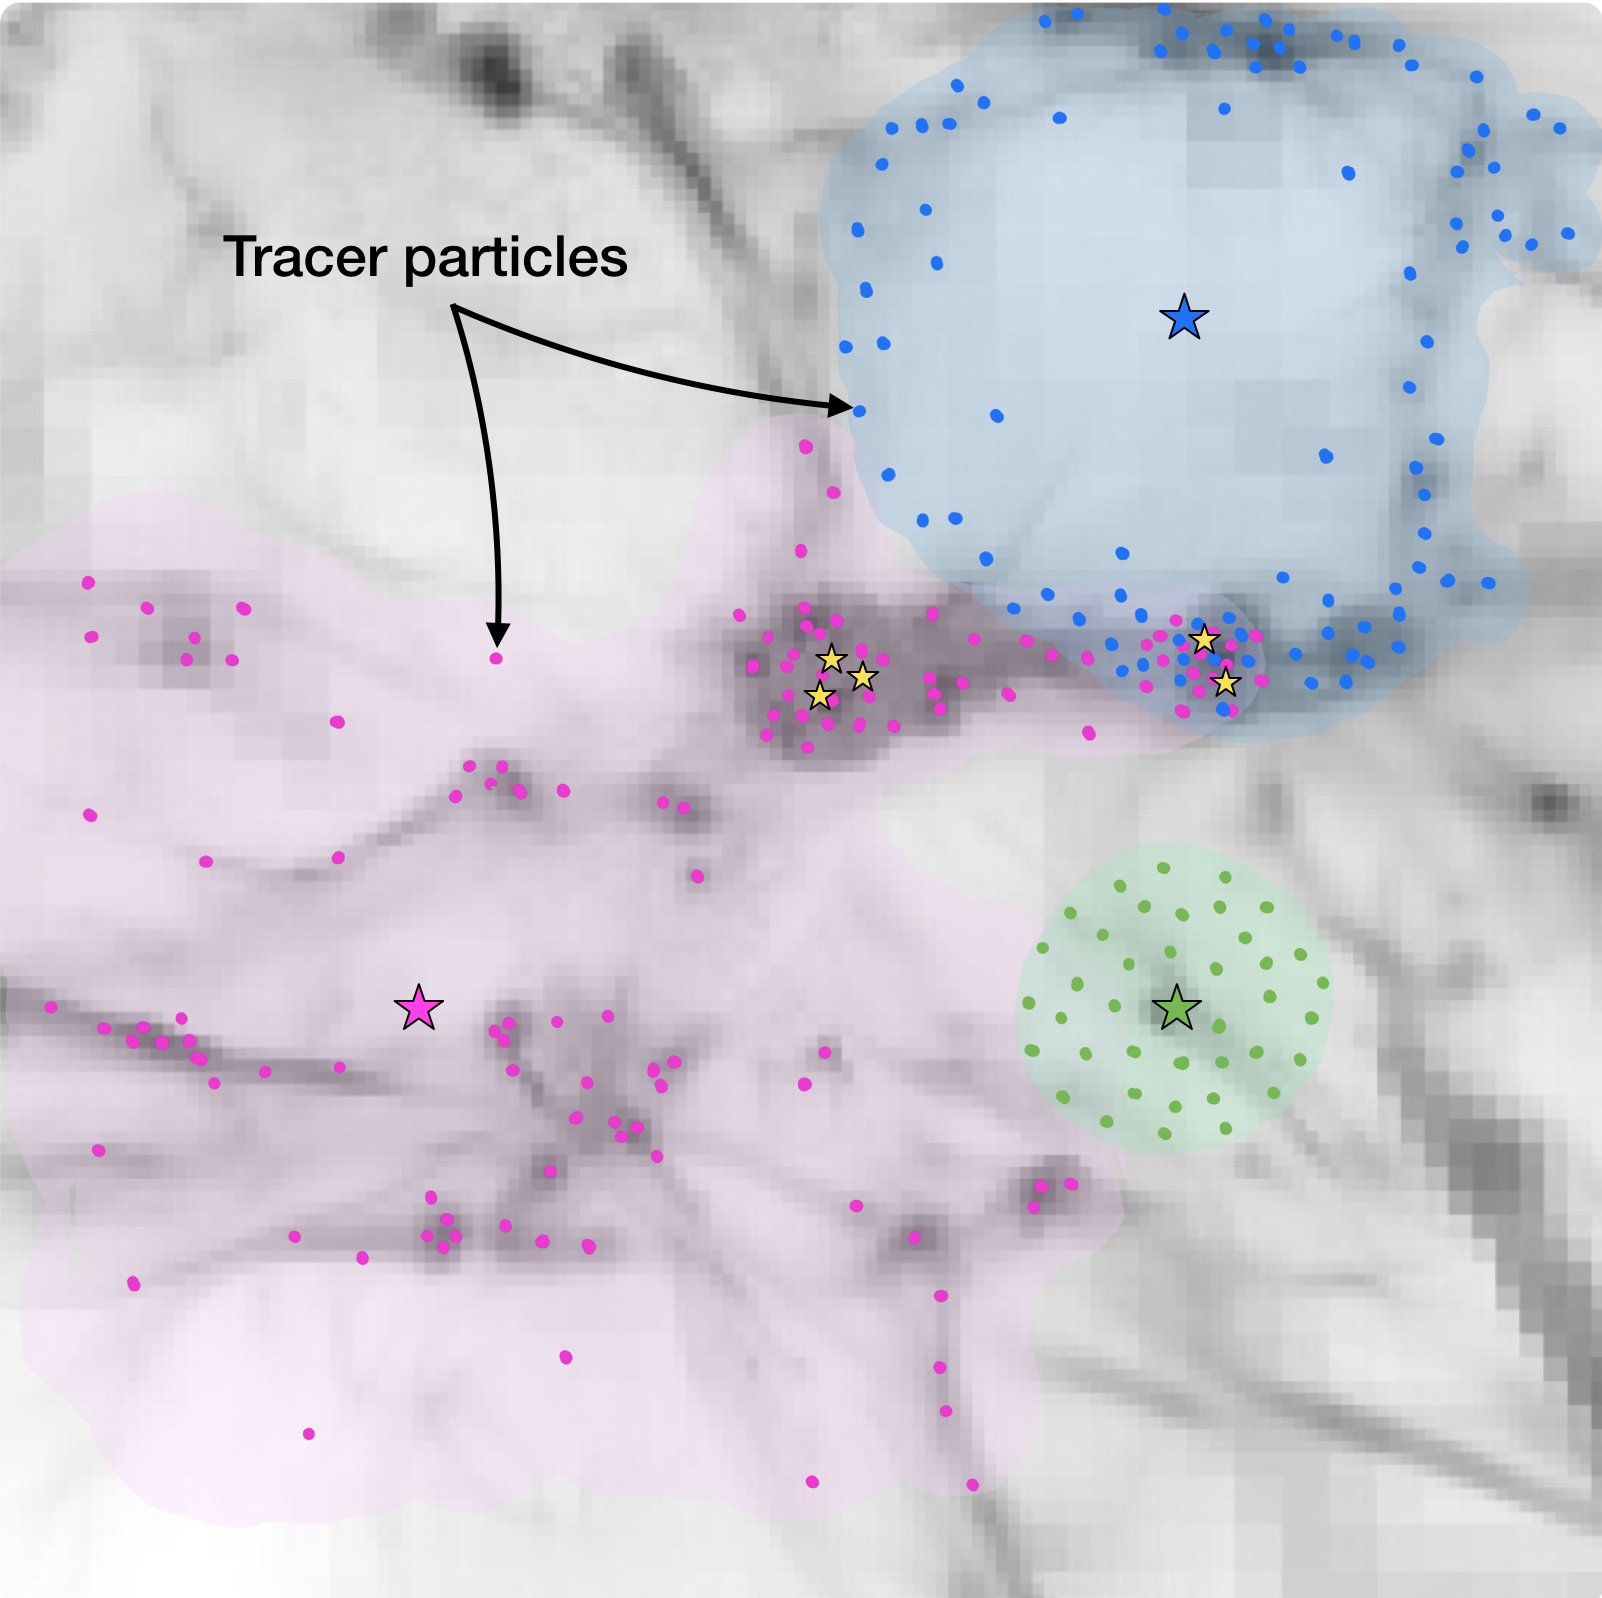
\includegraphics[width=0.6\textwidth]{figures/tracer_final}
%  \caption{Qualitative illustration of metal tracer particles. Black and white colors represent gas density in an example %cosmological simulation. Blue, pink, and green highlighted regions represent metal enrichment from the supernova remnants %of Pop III stars (blue, pink and green stars). Colored points represent tracer particles. Gold stars represent potential %sites of second-generation star formation. No stars are actually present in the example simulation.}
%  \label{fig:tracer}    
%\end{figure}


\subsection*{Access to Resources}

Our computational cosmology group has access to the PACE high-performance computing cluster at Georgia Tech, with 8 dedicated nodes, each with 28 cores, for our use only. We also have access to shared queues with 40,000 cores. These resources will be available to run our simulations and perform the necessary analyses. 

\subsection*{Project Timeline}
Each project is estimated to take approximately 1.5 years and produce at least one publication. In the first year, I will develop and run the triggered star formation simulation suite, set up a parallelized pipeline for efficient data analysis of many simulations simultaneously, and begin writing our first paper once the analysis is complete. In the second year, I will finish the first paper, develop the metal tracer particles in Enzo, generate the initial conditions for the cosmology simulations, run them, and begin to analyze the data. In the third year, I will finish analyzing the data for project 2, make publication-ready plots, and write our second paper.

\subsection*{Relevance to NASA's Science Mission Directive}
Together, the two projects put forth in this proposal will address the question of how we can relate the properties of the second-generation stars with first-generation, Population III stars. Additionally, this work has the power to explain the different formation channels and conditions that lead to the origin of Group II and Group III CEMP-no stars. On a more fundamental level, our simulations will provide a deep connection between the metal-free universe and the one we see today, enriched by metals from the first stars. \textbf{Both of these projects are in direct alignment with NASA's Science Mission Directive for the "Cosmic Origins" section of the Astrophysics Research Program.} We share the same goals of discovering how stars form within galaxies and discovering how these complex systems create and shape the structure and composition of the universe on all scales. Our cosmology simulations address these questions on the largest scales, and our triggered star formation simulations investigate these questions on smaller scales within individual galaxies. The timing of this research is optimal because our simulations and analysis will explicitly support NASA's future missions with the upcoming James Webb Space Telescope (JWST). JWST will be able to see deeper into the young, metal-poor universe than any previous telescope and study the environments in which the second-generation stars form. Our simulations will provide predictions for what JWST will see and aid in the interpretations of the observations. Specifically, we can make predictions about the metal content and distribution of galaxies in the early universe. Broadly speaking, since the first metals formed in the first stars, this research will bring us one step closer to understanding one of NASA's most fundamental questions, how did we get here?

\bibliography{proposal}

%%%%%%%%%%%%%%%%%%%%%%%%%%%%%%%%%%%%%%%%%%%%%%%%%%%%%%%%%%%%%%%%%%%%%%%%%%%%%%%%%%%%%%%%
% END Science/Technical/Management Section
%%%%%%%%%%%%%%%%%%%%%%%%%%%%%%%%%%%%%%%%%%%%%%%%%%%%%%%%%%%%%%%%%%%%%%%%%%%%%%%%%%%%%%%%

\section*{Acknowledgements}
This proposal was written entirely by me, Corey Brummel-Smith (FI). I received suggestions from my advisor Dr. John Wise (PI) and the professor of my grant writing class, Dr. Simon Sponberg, in the Georgia Tech School of Physics. I also allowed a few of my peers to look over my proposal and I took their feedback into account. I edited the text based on the suggestions of the persons above which helped me improve the grammar, clarity, and structure of the proposal.

\end{document}
